\documentclass[12pt,letterpaper]{article}

\newenvironment{proof}{\noindent{\bf Proof:}}{\qed\bigskip}

\newtheorem{theorem}{Theorem}
\newtheorem{corollary}{Corollary}
\newtheorem{lemma}{Lemma} 
\newtheorem{claim}{Claim}
\newtheorem{fact}{Fact}
\newtheorem{definition}{Definition}
\newtheorem{assumption}{Assumption}
\newtheorem{observation}{Observation}
\newtheorem{example}{Example}
\newcommand{\qed}{\rule{7pt}{7pt}}

\newcommand{\assignment}[4]{
\thispagestyle{plain} 
\newpage
\setcounter{page}{1}
\noindent
\begin{center}
\framebox{ \vbox{ \hbox to 6.28in
{\bf CS446: Machine Learning \hfill #1}
\vspace{4mm}
\hbox to 6.28in
{\hspace{2.5in}\large\mbox{Problem Set #2}}
\vspace{4mm}
\hbox to 6.28in
{{\it Handed Out: #3 \hfill Due: #4}}
}}
\end{center}
}

\newcommand{\solution}[4]{
\thispagestyle{plain} 
\newpage
\setcounter{page}{1}
\noindent
\begin{center}
\framebox{ \vbox{ \hbox to 6.28in
{\bf CS446: Machine Learning \hfill #4}
\vspace{4mm}
\hbox to 6.28in
{\hspace{2.5in}\large\mbox{Problem Set #3}}
\vspace{4mm}
\hbox to 6.28in
{#1 \hfill {\it Handed In: #2}}
}}
\end{center}
\markright{#1}
}

\newenvironment{algorithm}
{\begin{center}
\begin{tabular}{|l|}
\hline
\begin{minipage}{1in}
\begin{tabbing}
\quad\=\qquad\=\qquad\=\qquad\=\qquad\=\qquad\=\qquad\=\kill}
{\end{tabbing}
\end{minipage} \\
\hline
\end{tabular}
\end{center}}

\def\Comment#1{\textsf{\textsl{$\langle\!\langle$#1\/$\rangle\!\rangle$}}}


\usepackage{graphicx}
\oddsidemargin 0in
\evensidemargin 0in
\textwidth 6.5in
\topmargin -0.5in
\textheight 9.0in

\begin{document}

\solution{Nikhil Unni}{\today}{4}{Fall 2014}


\pagestyle{myheadings}  % Leave this command alone

\begin{enumerate}
\item
    \begin{enumerate}
    \item [a.] It's pretty easy to see that the VC dimension of the circle is at least 3. I've included a diagram to illustrate. In the diagram, the two inside points represent positive examples, while the outside is negative, as per the definition. Although it's only 1 example out of a possible 8, I think it's pretty easy to visualize... you can translate and scale the circle (in fact... just translate) to surround any 1, 2, or 3 points you need.
    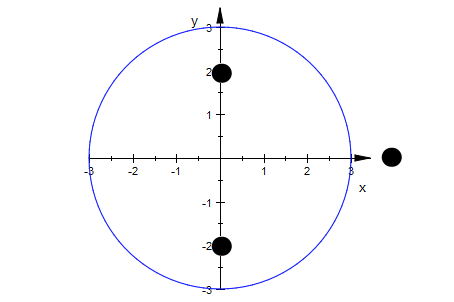
\includegraphics[scale=0.5]{circle}\\
    It's harder to show that the VC dimension cannot be 4, but there are some representative examples that suggest strongly that the VC dimension will be less than 4. (1) If all the points are collinear, the plus, minus, plus, minus orientation obviously cannot be shattered. (2) If the shape of the 4 points is a triangle (the convex hull, that is), there's a configuration of positives and negatives such that the ``fourth" point would be misclassified by a circle. (3) If the shape of the 4 points is some quadrilateral, and the opposite corners of the outline are the same label, there's no way the circle can ``stretch" to capture it (it's NOT an oval)! Because the VC dimension is greater than or equal to 3, and less than 4, it has to be 3.
    \item [b.] If you alternate +,-,+,-,...,+, with 2k points, there are k ``barriers'' needed between the + and -, since there k pairs of (+,-). So, for example, if k = 4, see the diagram:
    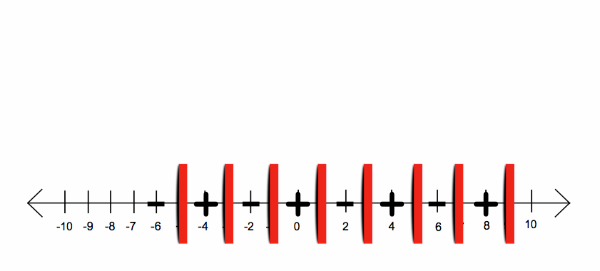
\includegraphics[scale=0.5]{number-line}\\
    This means the VC dimension is greater than or equal to 2k. But if I were to add an extra positive value to the left of -6, there would be no way to separate it from its closest negative point, meaning that the VC dimension is less than 2k+1, making its VC dimension 2k.
    \end{enumerate}
\item 
    \begin{enumerate}
    \item [a.] Negating a concept that can be represented as a k-decision list is pretty easy -- you just need to negate all of the booleans. Given $c = <(c_1,b_1), \ldots, (c_l,b_l), b>$, then $\neg c = <(c_1,\neg b_1), \ldots, (c_l,\neg b_l), \neg b>$
    \item [b.] Because all negations of concepts represented by the k-decision list can also be represented by k-decision lists, we only need to show that k-DNF $\subseteq$ k-DL. And this is easy to show since all k-DNFs can be converted to k-DL. Just take each term in the k-DNF and make it a node in the k-DL, with a label of 1, with a default value of 0. This is just because DNF acts as a ``cache'' of sorts, just memorizing key/value pairs. Because k-DNF $\subseteq$ k-DL, and we can represent negations, then k-DNF $\cup$ k-CNF $\subseteq$ k-DL.
    \item [c.] \underline{Algorithm}
    
    \begin{algorithm}
        1. Generate set of all possible conjunctions of the 2n literals of the input space,\\ from sizes 1 to k. (e.g. $x_1 \neg x_2$ or $x_1 x_2 x_3 x_4 $)\\
        2. while input data is not empty:\\
        3. \>\> Iterate through conjunction set until consistent conjunction, x, \\                  \>\>with input data. For example, a conjunction $x_2$ consistent   \\                \>\> with data: $([1,1,0,1],0), ([0,1,0,0],0)$ is consistent.\\
        4. \>\>Add $(x,c)$ to the outgoing decision list, where $c$ is the consistent label\\ 
           \>\>we found in step 3.\\
        5. \>\> Remove all examples from input data that matched the consistent conjunction.\\
        6. Return outgoing decision list.\\
    \end{algorithm}
    \item [d.] The size of our k-decision list is given by $O(n^k)$, for an input size of $n$. This gives us an approximate bound of $m > \frac{1}{\epsilon}(n^k + ln(\frac{1}{\delta}))$, which is polynomial in $n$, $\frac{1}{\epsilon}$, and $\frac{1}{\delta}$. So it is PAC-learnable. Furthermore, the algorithm used to generate it is $O(mn^k)$ (for each of the $\sum \limits_{i=1}^k {n \choose i}$ conjunctions, we iterated through the remaining examples in the training data), which is also polynomial in $n$.
    \end{enumerate}
\item 
    \begin{enumerate}
    \item [a.] $K(x_1,x_2) = \sum \limits_{i=0}^k {same(x_1,x_2) \choose i}$. This can be computed in linear time to n, since it just needs to calculate ``same'', which will just iterate through the features and compare the two.
    \item [b.] \underline{Kernel Perceptron Algorithm}
    \begin{algorithm}
        1. $\alpha$ = $\vec{0}$\\
        2. Repeat until convergence:\\
        3. \>\> Get next example, $(x_i,y_i)$\\
        4. \>\>If $(\sum \limits_{i=1}^n \alpha_i y_i \sum \limits_{j=0}^k {same(x_i,x) \choose j}) \neq y_i$:\\
        5. \>\>\> $\alpha_i = \alpha_i + 1$
    \end{algorithm}
    \item [c.] 
        Since we have blown up our original feature space from $n$ to some space $O(n^k)$, the mistake bound also significantly increases. Plugging into Novikoff's theorem, I got that the error bound, $M < 2^k$.
    \end{enumerate}
\end{enumerate}

\end{document}

